\chapter{Blocks Description}

%\section{AJIT Core}

%- Need to add the ajit expanded core diagram with debug ports labelled.

%\begin{figure}[H]
%\centering
%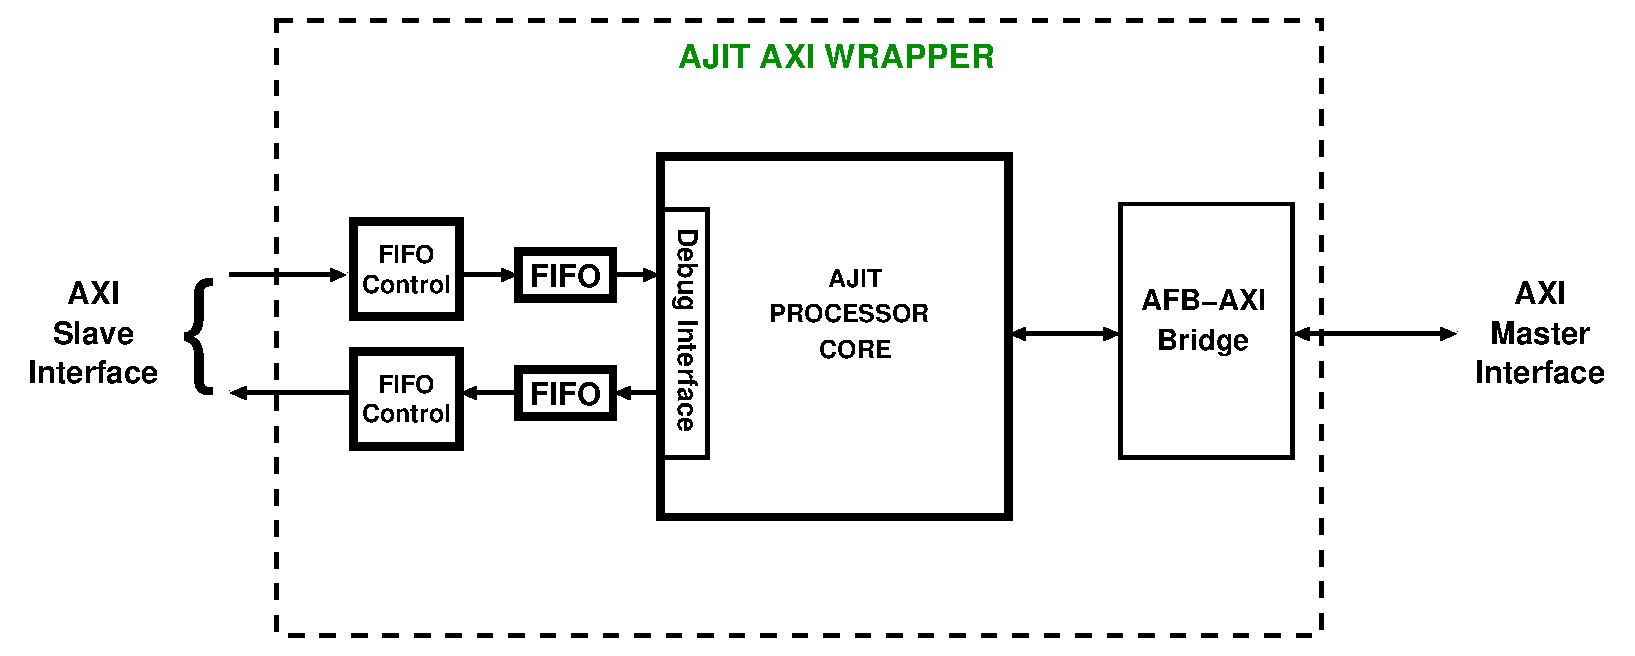
\includegraphics[scale=0.6]{eps_pdf_sources/ajit_fpga/System_Level/ajit_combined}
%\caption{AJIT AXI Wrapper}
%\label{ajit_combined}
%\end{figure}

\section{DRAM Controller}

\subsection{Need for a DRAM interface}

In the previous iteration of OS booting on AJIT processor the OS utilized the block RAM of the processor which was of size 4 MB
and thus took awhile to boot and only a small scale OS without much driver support(like Network drivers) could be booted, thus a need for a
larger DRAM support.  Here we head out to utilize the onboard DRAM of the VC709 board based on the ideas of our generic peripheral
interface discussed before.

\subsection{Our implementation}

The figure~\ref{DRAM Controller integrated flow} below shows our DRAM interface implementation as part of a generic AXI peripheral system.
DRAM interfaces with the AXI interconnect with the aid of a Memory Controller specifically employed for DRAMs. Memory controller was
generated using the MIG (Memory Interface Generator) utility of Vivado 2017.1. 

The support for DRAM size here goes up to 4 GB per slot and since VC709 has two slots we can have a combined support up to 8GB RAM.

\begin{figure}[H]
\centering
\includegraphics[width=\textwidth]{eps_pdf_sources/ajit_fpga/DRAM_without_PCIe/DRAM_without_PCIe}
\caption{DRAM Controller integrated flow}
\label{DRAM Controller integrated flow}
\end{figure}

\subsection{MIG Vs EMC Core}

The two cores provided in Vivado are for different types of memory. The following information can be found in the respective user guides
which summarise their use cases:

\begin{table}[H]
\centering
\begin{tabular}{c | c}
\hline
Core & Memory Support \\
\hline
 MIG & DDR2, DDR3, QDR-II, RLDRAM \\
 EMC & SRAM, ZBT, and other similar SRAM like interfaces \\
\end{tabular}
\caption{Comparison of Memory Cores}
\end{table}

\subsection{Testing of Interface}

We tested the interface using the XSCT command line utility which employs the JTAG interface and gives a direct access to all AXI
peripherals. Later on we also tested this with a PCI express interface from the Host CPU using the pcimem utility.

\section{PCIe-AXI IP}

\subsection{Need for a PCIe interface}

In the previous iteration of OS booting on AJIT processor the OS utilized the block RAM of the processor which was of size 4 MB
and the size of the kernel was just 2 MB and now as we increase the RAM size to accommodate a heavy duty OS we need a faster way to write
the image to the storage instead of JTAG and we are just in luck since VC709 has a PCIe interface and can be plugged directly into the PCIe
slot of the host CPU motherboard.  Right now we lack a flash interface in our system which would have allowed us to have a nonvolatile
memory block which would not require to be written at every power on-off cycle of the board. Here we utilize the PCIe interface of the
VC709 board.

\subsection{Basics of PCIe interface}

Before diving into the implementation details we need to revisit some essential basics of PCI express peripherals that would prove to be
useful here.  On a \textbf{Linux} machine one can type \verb|lspci -vv| in the console and get a detailed output of the PCIe devices
connected to the machine. Its a long list so I will explain with the example of the Xilinx's VC709 board. As can be seen from
listing~\ref{lst:lspci} the \verb|lspci| log gives out the details about the connected VC709 board's pci interface. Table~\ref{lspci
parameters} explains the relevant parameters in the \verb|lspci -vv| log.

\pagebreak

\singlespacing
\scriptsize{
\begin{lstlisting}[language=bash, caption=lspci log,label={lst:lspci}, emph={Region, lspci, vv, 0a:00\.0}]
$ lspci -vv
...
...
0a:00.0 Memory controller: Xilinx Corporation Device 7038 
        Subsystem: Xilinx Corporation Device 0007 
        Physical Slot: 3 
        Control: I/O+ Mem+ BusMaster- SpecCycle- MemWINV- VGASnoop- ParErr+ Steppi......
        Status: Cap+ 66MHz- UDF- FastB2B- ParErr- DEVSEL=fast >TAbort- <TAbort- <M......
        Interrupt: pin A routed to IRQ 16 
        Region 0: Memory at f0000000 (32-bit, non-prefetchable) [size=128M] 
        Region 1: Memory at e8000000 (32-bit, non-prefetchable) [size=128M] 
        Region 2: Memory at e0000000 (32-bit, non-prefetchable) [size=128M] 
        Region 3: Memory at d8000000 (32-bit, non-prefetchable) [size=128M] 
        Region 4: Memory at d0000000 (32-bit, non-prefetchable) [size=128M] 
        Region 5: Memory at c8000000 (32-bit, non-prefetchable) [size=128M] 
        Capabilities: <access denied> 
        Kernel modules: riffa
\end{lstlisting}
}

\begin{table}[H]
\centering
\begin{tabular}{c | c}
\hline
Parameter & Value\\
\hline
PCIe slot name & 0a:00.0 \\
Class & Memory Controller\\
Device id & 7038 \\
Physical slot & 3 \\
ProgIf & Region \textit{X} \\
Kernel modules option & riffa
\end{tabular}
\caption{lspci parameter description}
\label{lspci parameters}
\end{table}

\normalsize
\doublespacing
\begin{flushleft}
\textit{X is an integer from 0 to 5\\}
\textit{ProgIf : Programming Interface\\}
\textit{Kernel Modules: Kernel module reporting that it is capable of handling the device (optional, Linux only) for example here riffa\\}
\textit{Device id : This comes in handy when there are mulitple boards connected to the host}
\end{flushleft}

\subsection{BARs and address translation}

Whenever reading or writing we proceed with a method of providing a base address and the offset along with it which would amount to the
actual address.  We operate here with what is knows as BAR( Base Address Register ), it is the register which would hold the base/start
address of your Memory block which is DRAM here. One can make multiple BARs with different base addresses to access different parts of the
memory. Each BAR is set with a base address and an address range which it can access. Each bar created by the user gives rise to a new
resource file in the /sys/ directory of the host machine which as explained later in driver development can be used to access the respective
memory locations. The listing~\ref{lst:resource} shows the created resource files inside the \verb|/sys/bus/pci/devices/0000:0a:00.0/|
directory on the host machine in this case.

%\pagebreak

\singlespacing
\scriptsize{
\begin{lstlisting}[language=bash, caption=Resource files, label={lst:resource}, emph={root, irq, resource0, resource1, resource2, resource3, resource4, resource5}]
$ ä\textbf{ls -l /sys/bus/pci/devices/0000\:0a\:00.0/}ä
...
...
-r--r--r-- 1 root root      4096 Jun 18 15:30 irq
-rw------- 1 root root 134217728 Jun 18 16:17 resource0
-rw------- 1 root root 134217728 Jun 18 16:17 resource1
-rw------- 1 root root 134217728 Jun 18 16:17 resource2
-rw------- 1 root root 134217728 Jun 18 16:17 resource3
-rw------- 1 root root 134217728 Jun 18 16:17 resource4
-rw------- 1 root root 134217728 Jun 18 16:17 resource5
...
...
\end{lstlisting}
}
\normalsize
\doublespacing

\begin{flushleft}
134217728 \textit{bytes} = 128MB\\
\end{flushleft}

The \verb|irq| file provides memory mapped support for the interrupts received from the PCIe-AXI Translation IP on the FPGA system.
This could be later on used as an alternate to the current polling strategy of the custom PCIe driver as explained later.\\
The figure~\ref{PCIe flow} shows our PCIe-AXI interface implementation as part of a generic AXI peripheral system.  

\begin{figure}[H]
\centering
\includegraphics[width=\textwidth]{eps_pdf_sources/ajit_fpga/DRAM_with_PCIe/DRAM_with_PCIe}
\caption{PCIe-AXI interface and DRAM integrated design}
\label{PCIe flow}
\end{figure}

\subsection{Testing}

We tested this with a PCI express interface from the Host CPU using the pcimem utility. Later on we developed a C driver for creating an
API interface which provides helper functions for sending and receiving information through the PCIe-AXI interface to the FPGA model.

\section{AFB-AXI Bridge}

\subsection{Need for a Custom IP for AFB-AXI Interface}

AFB(AJIT FIFO Bus) is an in-house term coined to represent the data bus of AJIT which allows it to talk to other AXI peripherals. AFB is not
directly AXI compatible and thus needs a bridge, we developed it from scratch in Verilog keeping in mind the provided AFB specifications.

\subsection{Our implementation}

We generated a custom IP bridge by writing a Verilog file and then packaging an IP through Vivado's IP Manager to make it available in the
user repository in Vivado IP repository. The bridge supports AXI-Lite on one side and AFB on the other. As can be seen in
figure~\ref{AFB-AXI bridge} the input port on the left directly interfaces with the AJIT core and then passes on the input AJIT request to
the AFB parser block which then splits the request according to the AFB specs as mentioned before and packages it as AXI Master packets and
forwards the packets to the corresponding AXI bridge's FIFOs i.e. write address, write data and read address. It also reads the response
FIFO and the read data FIFO and packages the AXI FIFO's data back into the AFB response format and sends it back to AJIT core.

\begin{figure}[H]
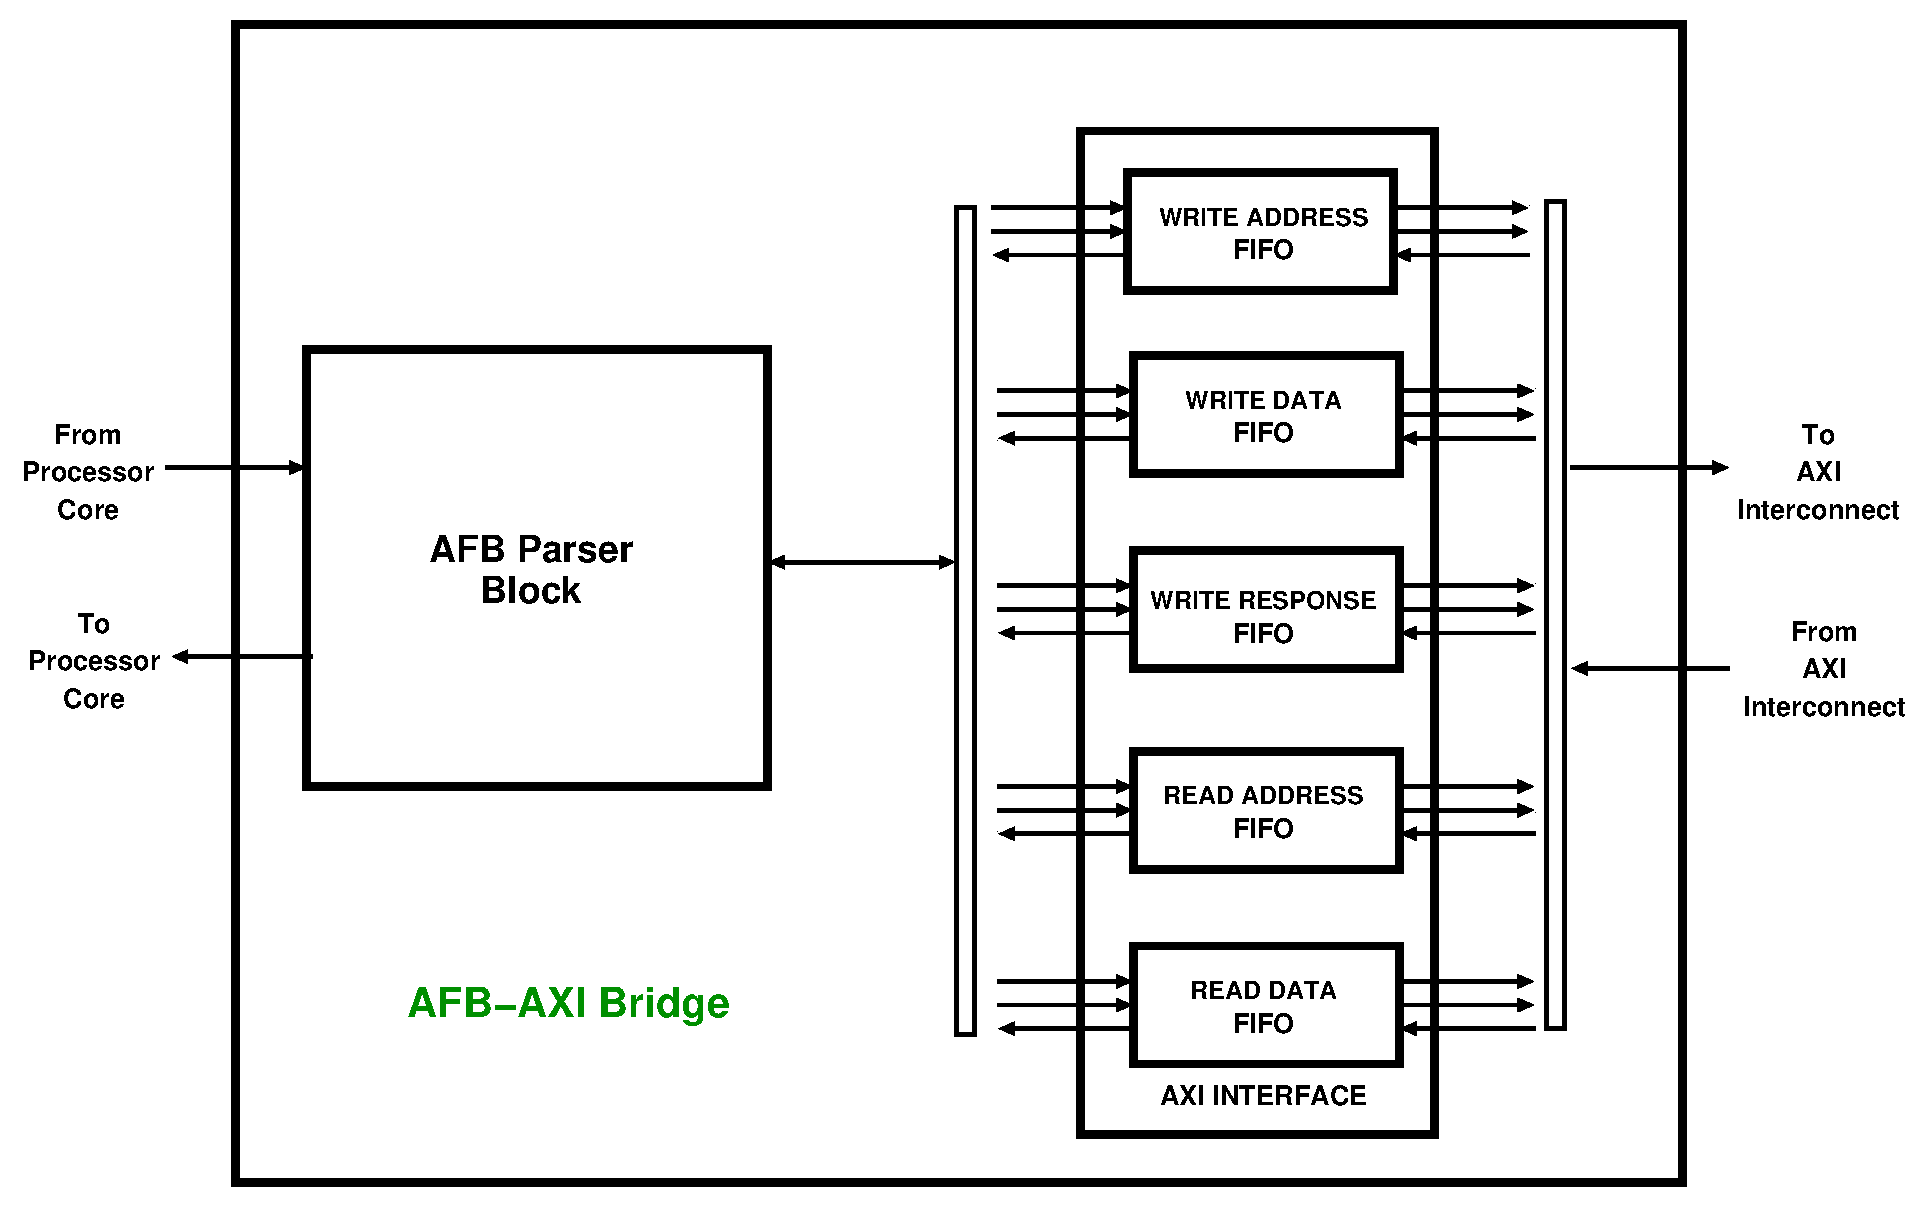
\includegraphics[width=\textwidth]{eps_pdf_sources/ajit_fpga/AFB_AXI_bridge/AFB_AXI_bridge_expanded}
\caption{AFB-AXI Bridge}
\label{AFB-AXI bridge}
\end{figure}

\subsection{Full Flow}

The figure below shows the full flow model integrated with the AFB-AXI bridge.

\begin{figure}[H]
\centering
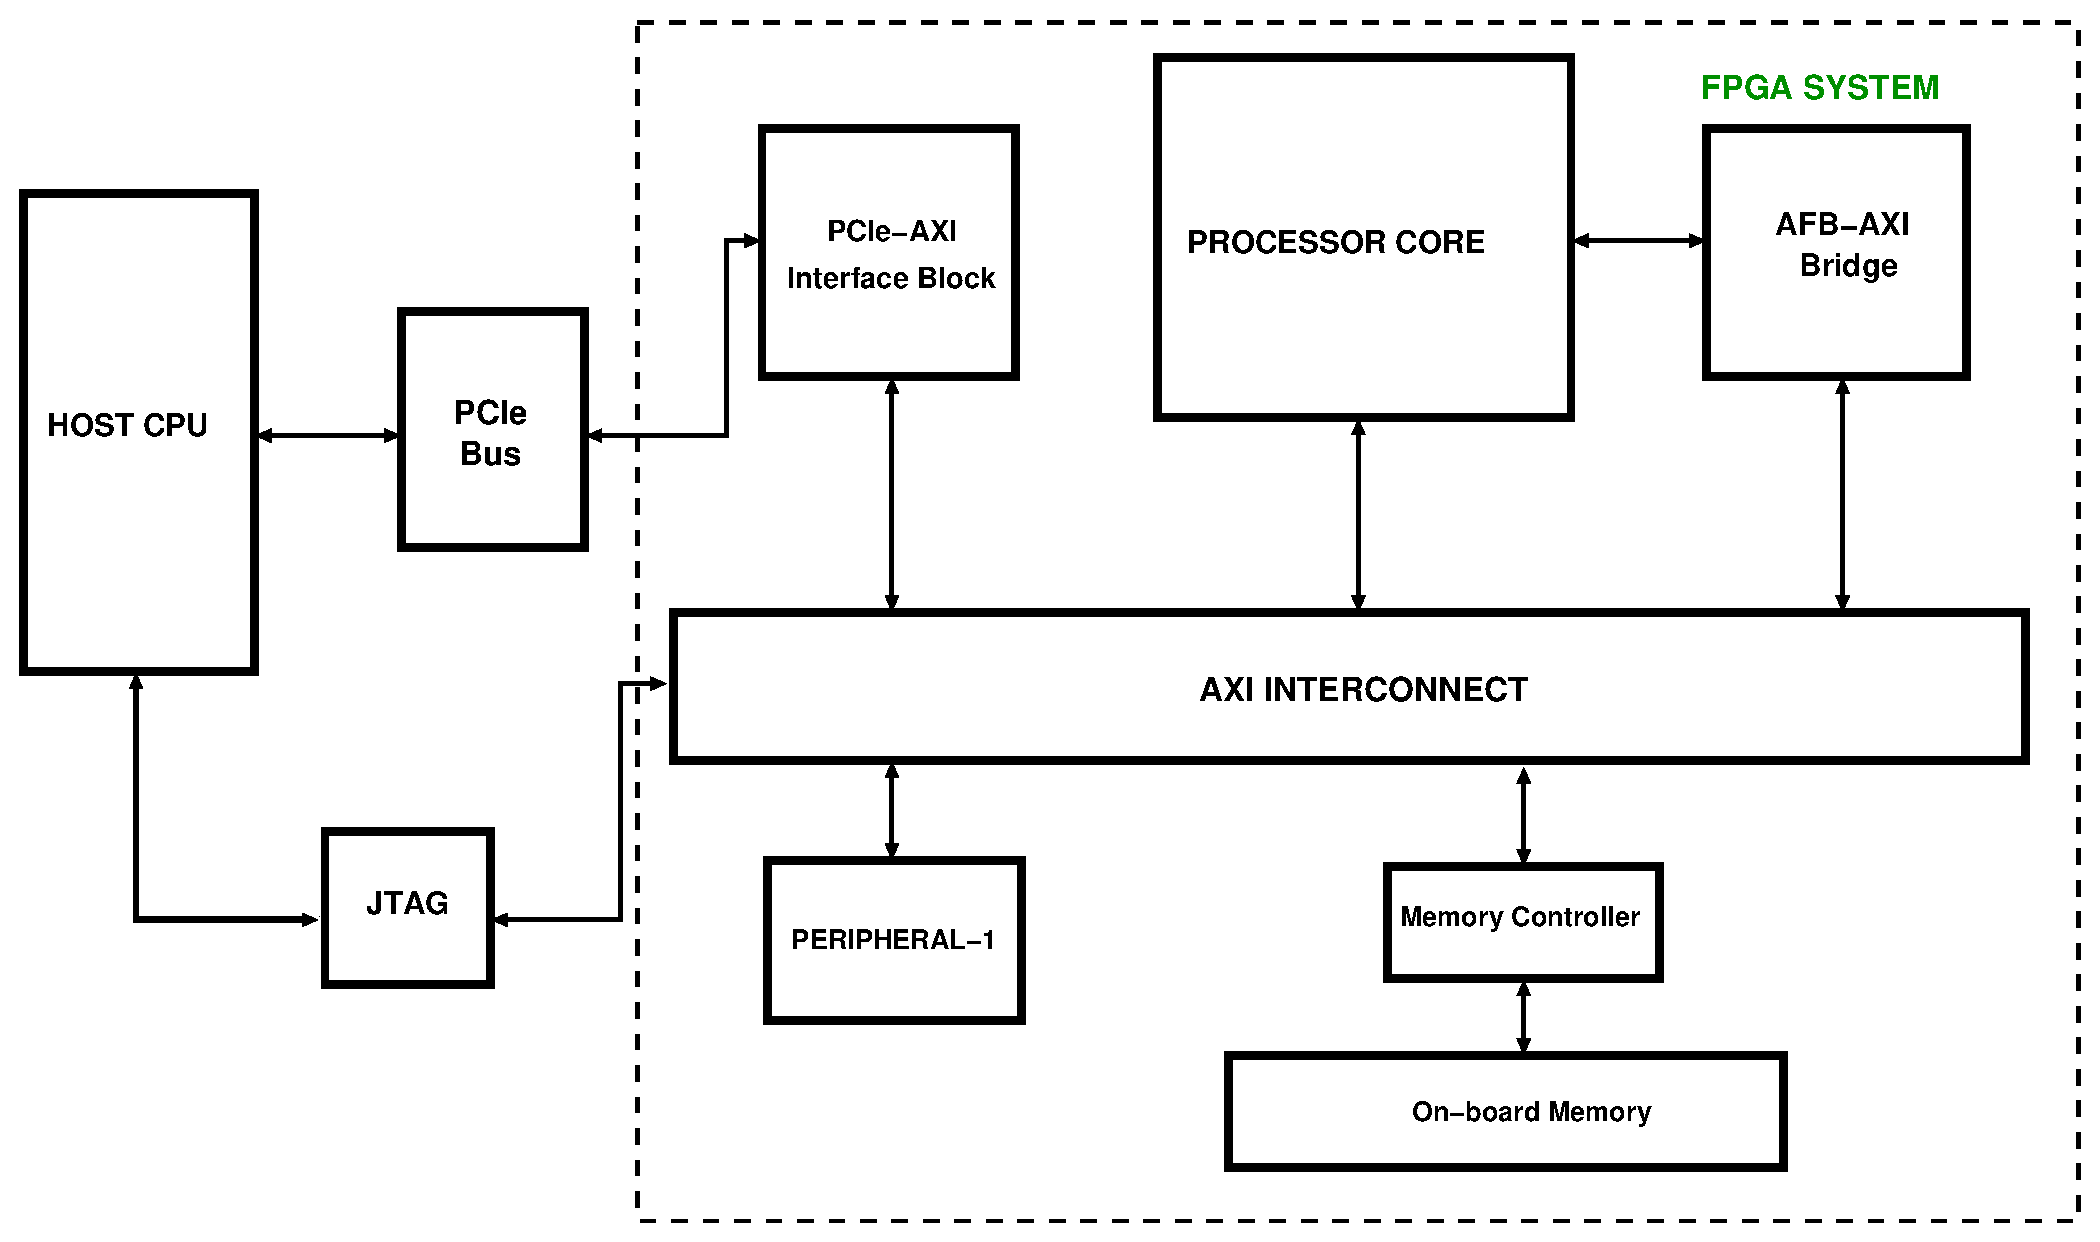
\includegraphics[width=\textwidth]{eps_pdf_sources/ajit_fpga/AFB_AXI_bridge/AFB_AXI_bridge_integrated}
\caption{Flow with AFB-AXI Bridge}
\end{figure}

\subsection{Testing of Interface}

We conducted manual memory read-write tests on the interface using the XSCT command line utility which employs the JTAG interface and gives
a direct access to all AXI peripherals. Later on we also tested this with a PCI express interface from the Host CPU using the pcimem
utility.

\section{FIFOs }

Figure~\ref{fifo} shows the generic FIFO interface generated by AHIR which has been used at almost all interfaces in the FPGA system design.
The AXI side interface \verb|hls_stream| though uses a similar FIFO but with READY and ACCEPT signals instead of REQ and ACK. The timing
diagram for the same has been shown in figure.%~\ref{}.

\begin{figure}[H]
\centering
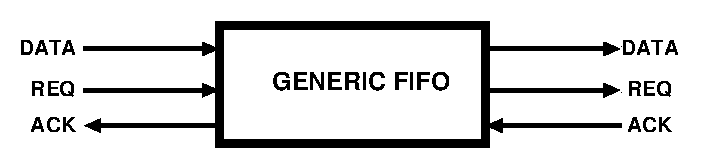
\includegraphics[width=\textwidth]{eps_pdf_sources/ajit_fpga/AFB_AXI_bridge/FIFO}
\caption{Generic FIFO Interface}
\label{fifo}
\end{figure}

\section{FIFO Controllers}

\subsection{Need for a Memory Mapped FIFO}

The Debug interface to the processor requires two 64-bit FIFOs compatible with the generic AXI peripheral interface. Here by compatibility
we mean they need to have a Slave AXI interface in order to establish a bidirectional data flow through the PCIe-AXI interface.

The problem is solved by dividing it into two parts and both of them handling simpler generic tasks. The first block provides the Slave AXI
interface as an input and a control interface on the output side to the other block which acts as a data FIFO. A similar block is created to
perform the reverse operation as well.

\subsection{Our implementation}

%\onehalfspacing
We employ \textbf{Vivado HLS}(High Level Synthesis) to generate the FIFO controllers. This enables us to write short code snippets as shown
in listing~\ref{lst:fifo controller hls} to generate the Slave AXI data interface and control signals for the FIFO controller which would
read AJIT's response from the FIFO and write it in it's slave register. The cpp template \verb|hls_stream| generates the FIFO compatible
interface so that the controller can en-queue and de-queue the debug FIFO.  Table~\ref{pragma description} provides explanation for the important
\verb|pragma| statements.

\pagebreak

\scriptsize
\singlespacing
\begin{lstlisting}[language=C++, caption=FIFO Controller HLS, label={lst:fifo controller hls}]
void fifo_to_axi_slave (ap_uint<32> data_out, ..., hls::stream<ap_uint<32> > &in_fifo) {
    #pragma HLS INTERFACE s_axilite port=return
    #pragma HLS INTERFACE s_axilite port=data_out
    #pragma HLS INTERFACE s_axilite port=data_valid
    if (!in_fifo.empty ()) {
        data_out   = in_fifo.read ();
        data_valid = true;
    }
    else {
        data_valid = false;
    }
}
\end{lstlisting}

\normalsize
\doublespacing

\begin{table}[H]
%\centering
\begin{tabular}{| l | l |}
\hline
Pragma Statement & Description\\
\hline
HLS INTERFACE s\_axilite port return & Generates the control signals (start, done etc.)\\
HLS INTERFACE s\_axilite port data\_out & Memory mapped register for read data\\
HLS INTERFACE s\_axilite port data\_valid & Memory mapped register for data valid signal\\
\hline
\end{tabular}
\caption{Pragma Statement Description}
\label{pragma description}
\end{table}

\subsection{Full Flow}

The figure~\ref{full system} shows our complete FPGA implementation as a generic AXI peripheral system. AJIT core interfaces with the DRAM controller
indirectly through the AFB-AXI bridge which translates its requests to the AXI format, AJIT interfaces to the host machine through the debug
interface which is also AXI compatible and is controlled by the host through the PCI-AXI translation bridge which is used to translate PCIe requests to AXI
requests but the interesting thing to note is that it can also be controlled by on-board master peripherals for example the processor. The
figure~\ref{full system with flow} shows the crucial data flows in the FPGA system.

\begin{figure}[H]
\centering
\includegraphics[width=\textwidth]{eps_pdf_sources/ajit_fpga/Full_System/Full_system}
\caption{Complete FPGA system}
\label{full system}
\end{figure}

\begin{figure}[H]
\centering
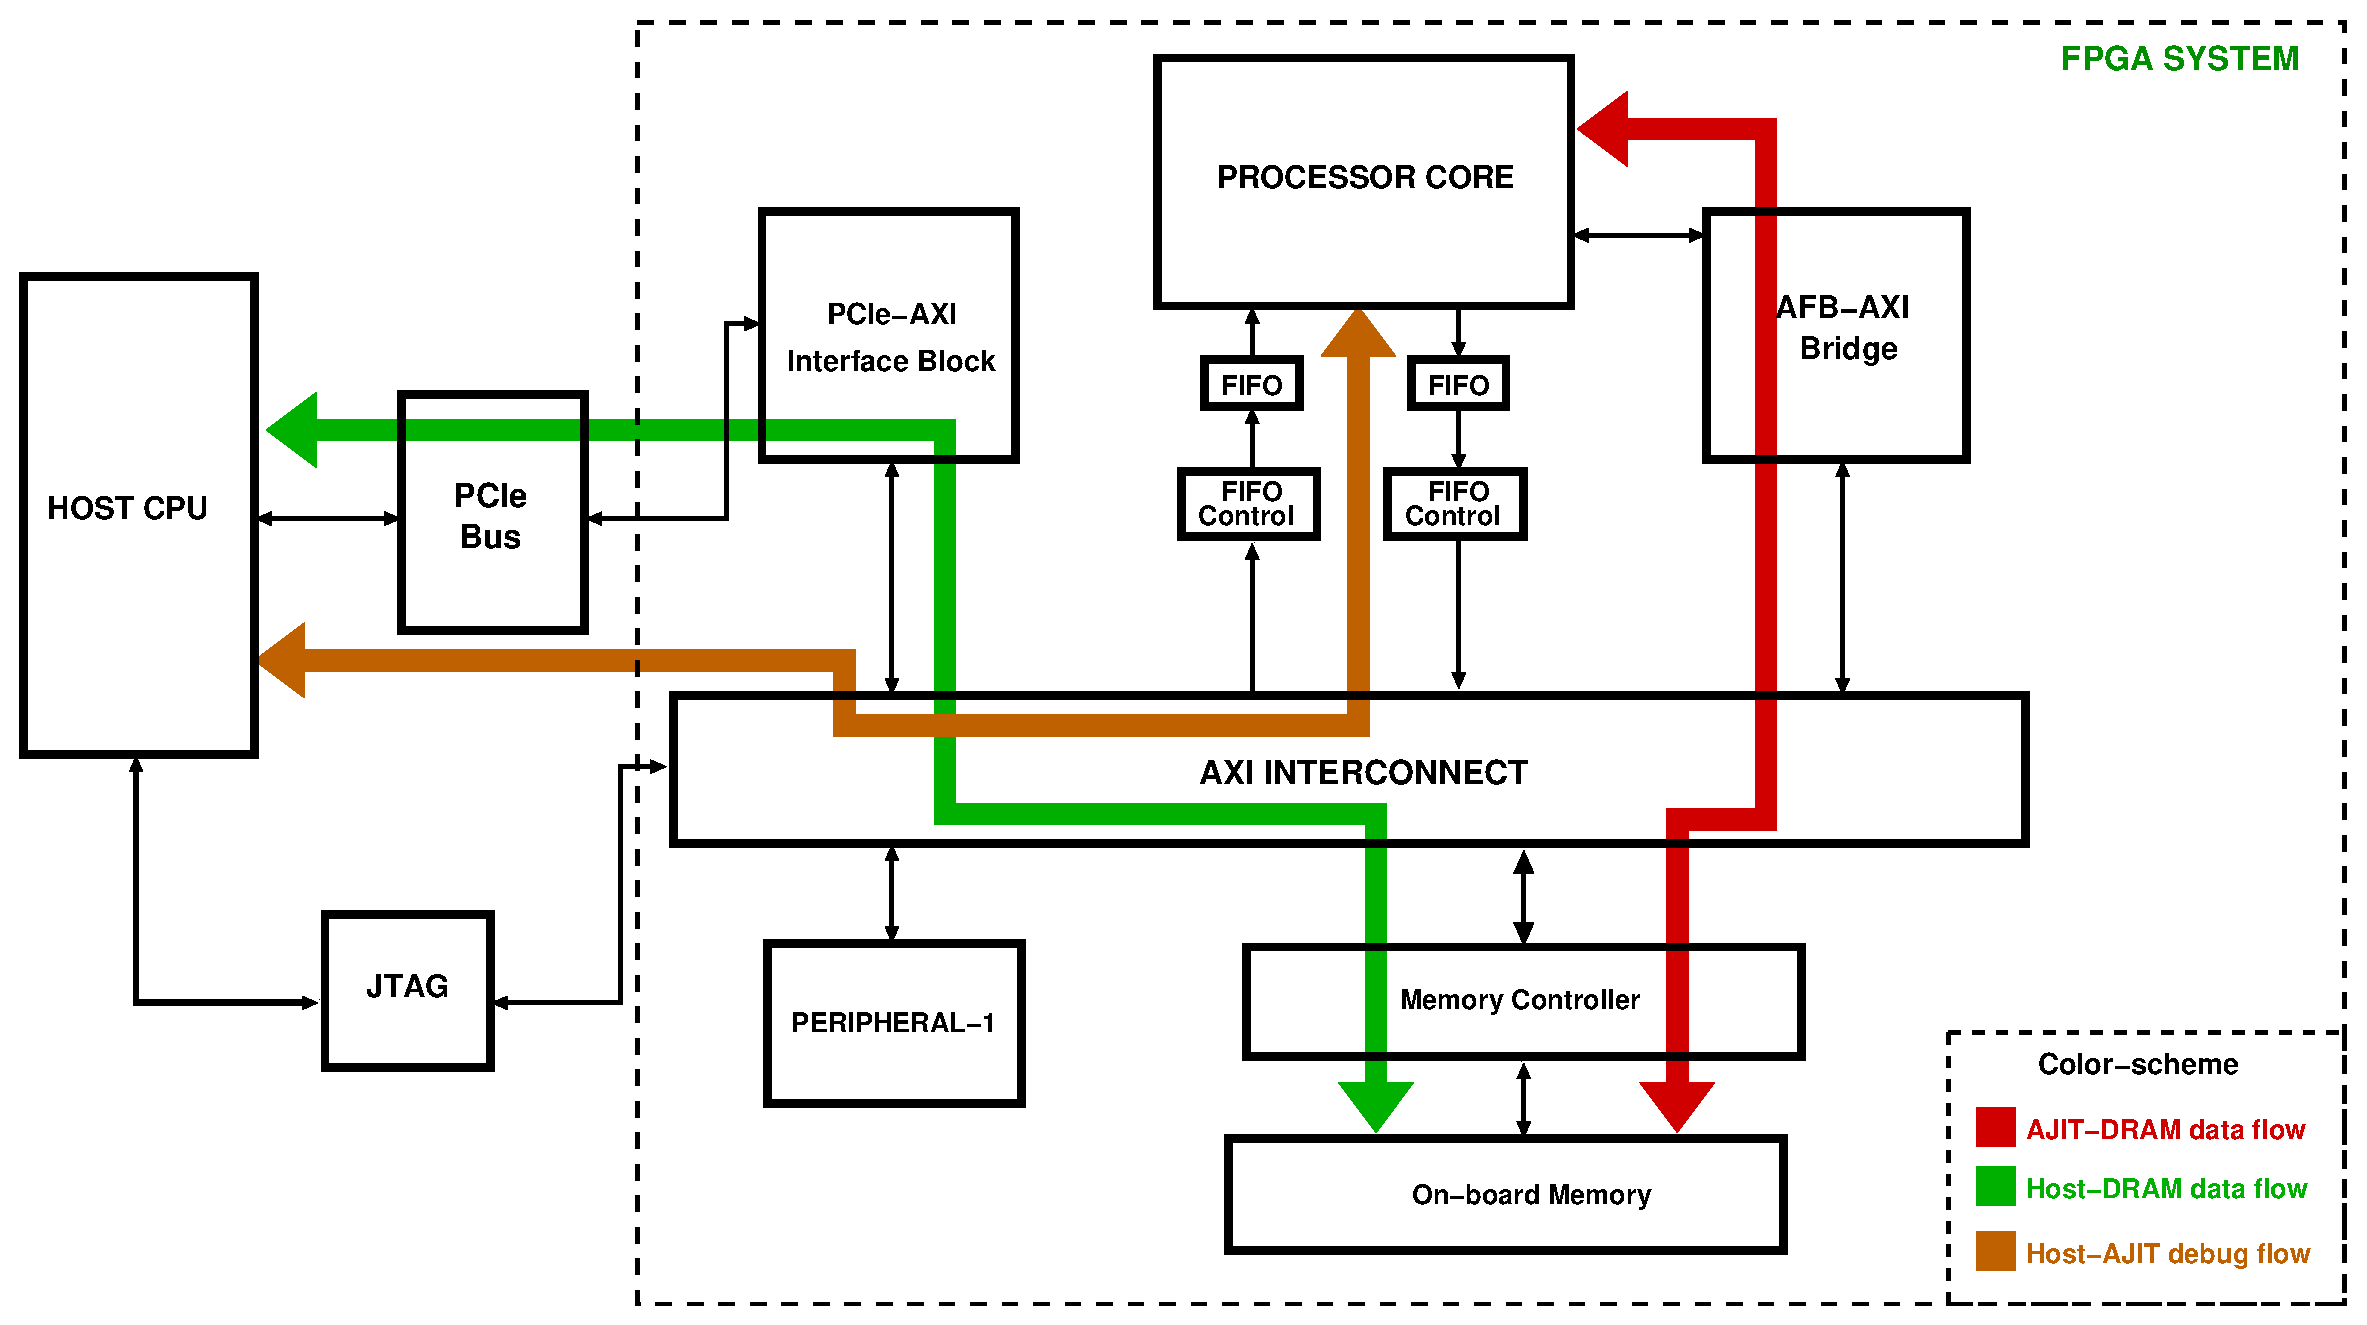
\includegraphics[width=\textwidth]{eps_pdf_sources/ajit_fpga/Full_System/Full_system_with_flow}
\caption{Complete FPGA system with data flow}
\label{full system with flow}
\end{figure}

\subsection{Testing of Interface}

We tested the interface using the XSCT command line utility which employs the JTAG interface and gives a direct access to all AXI
peripherals, an example of the same is shown in listing~\ref{lst:xsct}. 

\singlespacing
\scriptsize{
\begin{lstlisting}[language=bash, caption=xsct in action, label={lst:xsct}, emph={xsct, mrd, mwr}]
$ ä\textbf{xsct}ä
xsct% connect                                                                                                                                                             
attempting to launch hw_server
                                                                                                                                                                          
****** Xilinx hw_server v2017.1
  **** Build date : Apr 14 2017-19:01:52
    ** Copyright 1986-2017 Xilinx, Inc. All Rights Reserved.

INFO: hw_server application started
INFO: Use Ctrl-C to exit hw_server application

INFO: To connect to this hw_server instance use url: TCP:127.0.0.1:3121

tcfchan#0
xsct% target 3
xsct% mwr 0x80000000 0x01 
xsct% mrd 0x80000000
      0x01
\end{lstlisting}
}

\normalsize
\doublespacing

We also tested this with a PCI express interface from the Host CPU using the pcimem utility, an example of the same is shown in
listing~\ref{lst:pcimem}.

\singlespacing
\scriptsize{
\begin{lstlisting}[language=bash, caption=pcimem in action, label={lst:pcimem}, emph={resource0}]
$ ä\textbf{sudo ./pcimem /sys/bus/pci/devices/0000\:0a\:00.0/resource0 0 w}ä
  /sys/bus/pci/devices/0000\:0a\:00.0/resource0 opened.
  Target offset is 0x0, page size is 4096
  mmap(0, 134217728, 0x3, 0x1, 3, 0x0)
  PCI Memory mapped to address 0x4801f000.
  Value at offset 0x0 (0x4801f000): 0xC0BE0100
\end{lstlisting}
}
\normalsize
\doublespacing
